\documentclass[border=10pt]{standalone}
%%%<
\usepackage{verbatim}
%%%>
\begin{comment}
:Title: Polar plot of a sine function with factor in argument
:Tags: 2D;Functions;Polar Plots
:Author: Stefan Kottwitz
:Slug: sine-plot

The sine function is a well known periodic function. Choose an argument
factor, which doesn't divide the period well, and you can see a complicated
path around the origin.

This plot was originally made for my blog post on TikZ.de:
http://tikz.de/periodisch/

See also the other polar sine plot examples there.
\end{comment}
\usepackage{pgfplots}
\usepgfplotslibrary{polar,colormaps}
\begin{document}
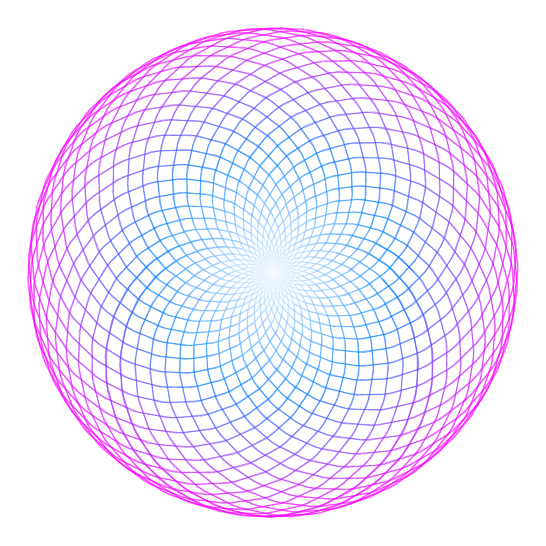
\begin{tikzpicture}
  \begin{polaraxis}[
      domain  = -14400:14400,
      samples = 3000,
      colormap/cool,
      hide axis
    ]
    \addplot[no markers, mesh, opacity=0.5] {1-sin(40*x/39};
  \end{polaraxis}
\end{tikzpicture}
\end{document}
